\documentclass[letterpaper]{article}
\usepackage[margin=1in]{geometry}
\usepackage[utf8]{inputenc}
\usepackage{amsmath}
\usepackage{amssymb}
\usepackage{mathrsfs} %for math script%
\usepackage{graphicx}
\usepackage{float}
%\usepackage{flafter}
%\usepackage{afterpage}
\usepackage{indentfirst}
\usepackage{hyperref}
\graphicspath{{figures/}}
\setlength{\parindent}{0pt}

\newcommand{\Dt}{\Delta t}
\newcommand{\Dx}{\Delta x}

\begin{document}

\section{ARZ model}

Consider the full nonlinear ARZ model without relaxation \cite{AR, Z}:
\begin{align} 
\rho_t + (\rho v)_x &= 0, \label{ARZ1} \\
(v - V(\rho))_t + v(v - V(\rho))_x &=0. \label{ARZ2}
\end{align}

\section{Explicit numerical schemes}

\subsection{Godunov}

The Godunov scheme requires a Riemann solver. To apply this scheme we first write the system in conservation form. The model is \cite{GodunovARZ}:
\begin{equation} \label{eq:consv}
U_t + [F(U)]_x = 0,
\end{equation}
with conserved variables $U = \begin{pmatrix} \rho \\ y \end{pmatrix}$ and flux vector $F(U) = \begin{pmatrix} y + \rho V(\rho) \\ \dfrac{y^2}{\rho} + y V(\rho) \end{pmatrix}$.

The scheme is 
\begin{equation}
U^{n+1}_j = U^n_j - \dfrac{k}{h}\left[F(u^*(U^n_j, \, U^n_{j+1})) - F(u^*(U^n_{j-1}, \, U^n_j))\right],
\end{equation}
where $u^*(U^n_j, \, U^n_{j+1})$ is the solution to the Riemann problem with initial data $U^n_j$ and $U^n_{j+1}$. The Riemann problem solution is discussed in \cite{GodunovARZ}.

\subsection{Lax-Friedrichs}
The Lax-Friedrichs scheme can be applied to equations in the form of \eqref{eq:consv} as well, but a Riemann solver is not needed. The partial derivatives are approximated using a forward difference in time and central difference in space, and $U^n_j$ is replaced with its spatial average. The scheme is:
\begin{equation}
U^{n+1}_j = \frac{1}{2}[U^n_{j+1} + U^n_{j-1}] - \dfrac{\Dt}{2 \Dx}[F(U^n_{j+1}) - F(U^n_{j-1})].
\end{equation}

This method is first-order accurate and very dissipative \cite{LeVequetext}. The stencil for this method is shown in Figure 
\ref{fig:stencil_laxfried}. \\

\begin{figure}[H]
\centering
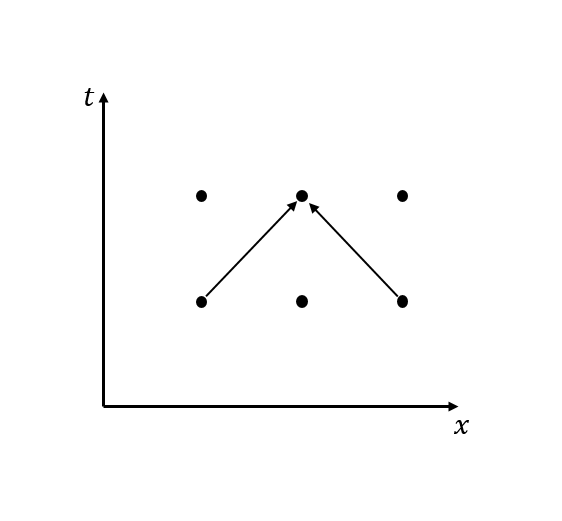
\includegraphics[trim = 10mm 20mm 10mm 15mm, width=0.3\textwidth]{Laxfried.png}
\caption{Stencil for Lax-Friedrichs method.}
\label{fig:stencil_laxfried}
\end{figure}


\subsection{Lax-Wendroff}
We look at a higher-order scheme with less numerical dissipation. For nonlinear conservation laws, the Lax-Wendroff scheme is: 
\begin{align}
U^{n+1}_j = U^n_j &- \dfrac{\Dt}{2 \Dx}[F(U^n_{j+1}) - F(U^n_{j-1})] + \dfrac{(\Dt)^2}{2 (\Dx)^2}[A_{j+1/2}(F(U^n_{j+1}) \notag \\ 
&- F(U^n_j)) - A_{j-1/2}(F(U^n_j)- F(U^n_{j-1}))],
\end{align}
where $A_{j\pm 1/2}$ is the Jacobian matrix $F'(\cdot)$ evaluated at $\frac{1}{2}(U^n_j + U^n_{j\pm1})$. Evaluating the Jacobian matrix makes this method more expensive to use so Richtmyer proposed a two-step procedure to avoid using $A$. In the first step $u(x,t)$ is calculated at half time and space steps. In the second step these values are used to compute the solution at the next time step. 

Richtmyer's two-step Lax-Wendroff method is: 

First step:
\begin{align}
U^{n+1/2}_{j+1/2} &= \dfrac{1}{2}(U^n_{j+1} + U^n_j - \dfrac{\Dt}{2 \Dx} [F(U^n_{j+1} - F(U^n_j)] \\
U^{n+1/2}_{j-1/2} &= \dfrac{1}{2}(U^n_j + U^n_{j-1} - \dfrac{\Dt}{2 \Dx} [F(U^n_j - F(U^n_{j-1})]
\end{align}
Second step:
\begin{equation}
U^{n+1}_j = U^n_j - \dfrac{\Dt}{\Dx}[F(U^{n+1/2}_{j+1/2}) - F(U^{n+1/2}_{j-1/2})]
\end{equation}

This method is second-order accurate and less dissipative than the Lax-Friedrichs method.  However, as the Lax-Wendroff method does not preserve monotonicity, it produces oscillations near discontinuities \cite{LeVequetext}. 

The stencil for this method is shown in Figure 
\ref{fig:stencil_laxwend}. \\

\begin{figure}[H]
\centering
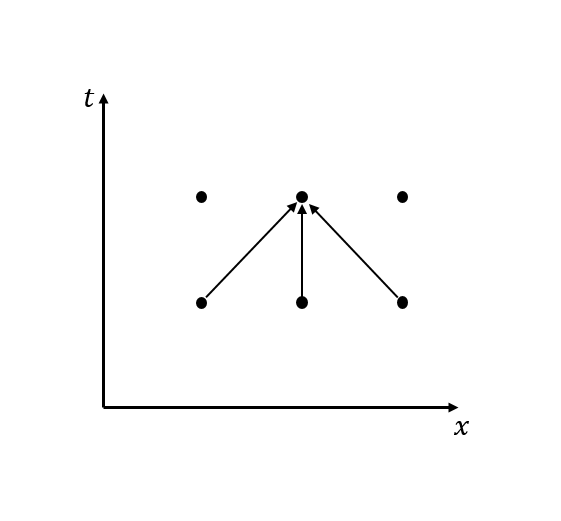
\includegraphics[trim = 10mm 20mm 10mm 15mm, width=0.3\textwidth]{Laxwend.png}
\caption{Stencil for Lax-Wendroff method.}
\label{fig:stencil_laxwend}
\end{figure}


\subsection{ENO and WENO}

The ENO (essentially non-oscillatory) schemes were developed by Harten, Engquist, Osher, and Chakravarthy to solve the problem of finding higher-order schemes that do not produce oscillations near discontinuities \cite{LeVequetext}. The idea is to use a high-degree polynomial to  interpolate the solution $U$, then compute $[F(U)]_x$. The stencil is chosen depending on the upwind direction. Points added for higher-order polynomials are chosen so that the interpolant has the least oscillation.

\begin{figure}[H]
\centering
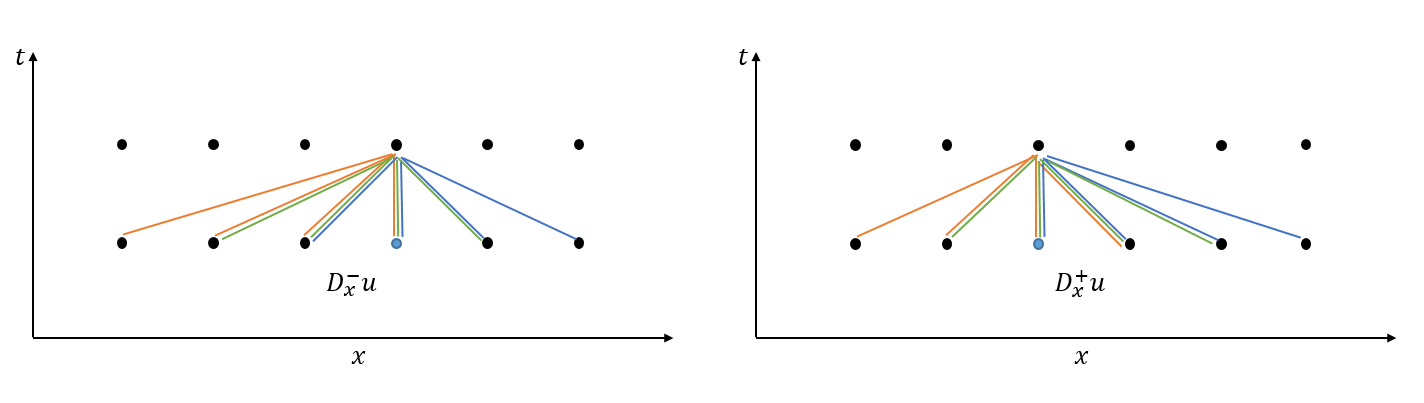
\includegraphics[width=160mm]{ENO.png}
\caption{Possible stencils for ENO represented by different colors. $D^-_x u$ is used if information propagates from left to right and $D^+_x u$ is used if information propagates from right to left.}
\label{fig:stencil_ENO}
\end{figure}

The WENO (weighted ENO) scheme, introduced by Liu, Osher, and Chan \cite{WENO}, uses a convex combination approach rather than picking the smoothest stencil in order to achieve the ENO property. Instead of using stencils as in ENO, WENO uses a weighted combination of higher-order reconstructions to approximate $U$. The weights depend on a smoothness indicator which estimates the smoothness of the solution. 

Both ENO and WENO schemes discretize in space. Essentially these schemes reconstruct $U$, then compute $[F(U)]_x$. TVD Runge-Kutta schemes can be used to solve in time for the solution. 

\section{Implementation of explicit schemes}
A comparison of the scheme with actual data is shown below. 

\begin{figure}[H]
\centering
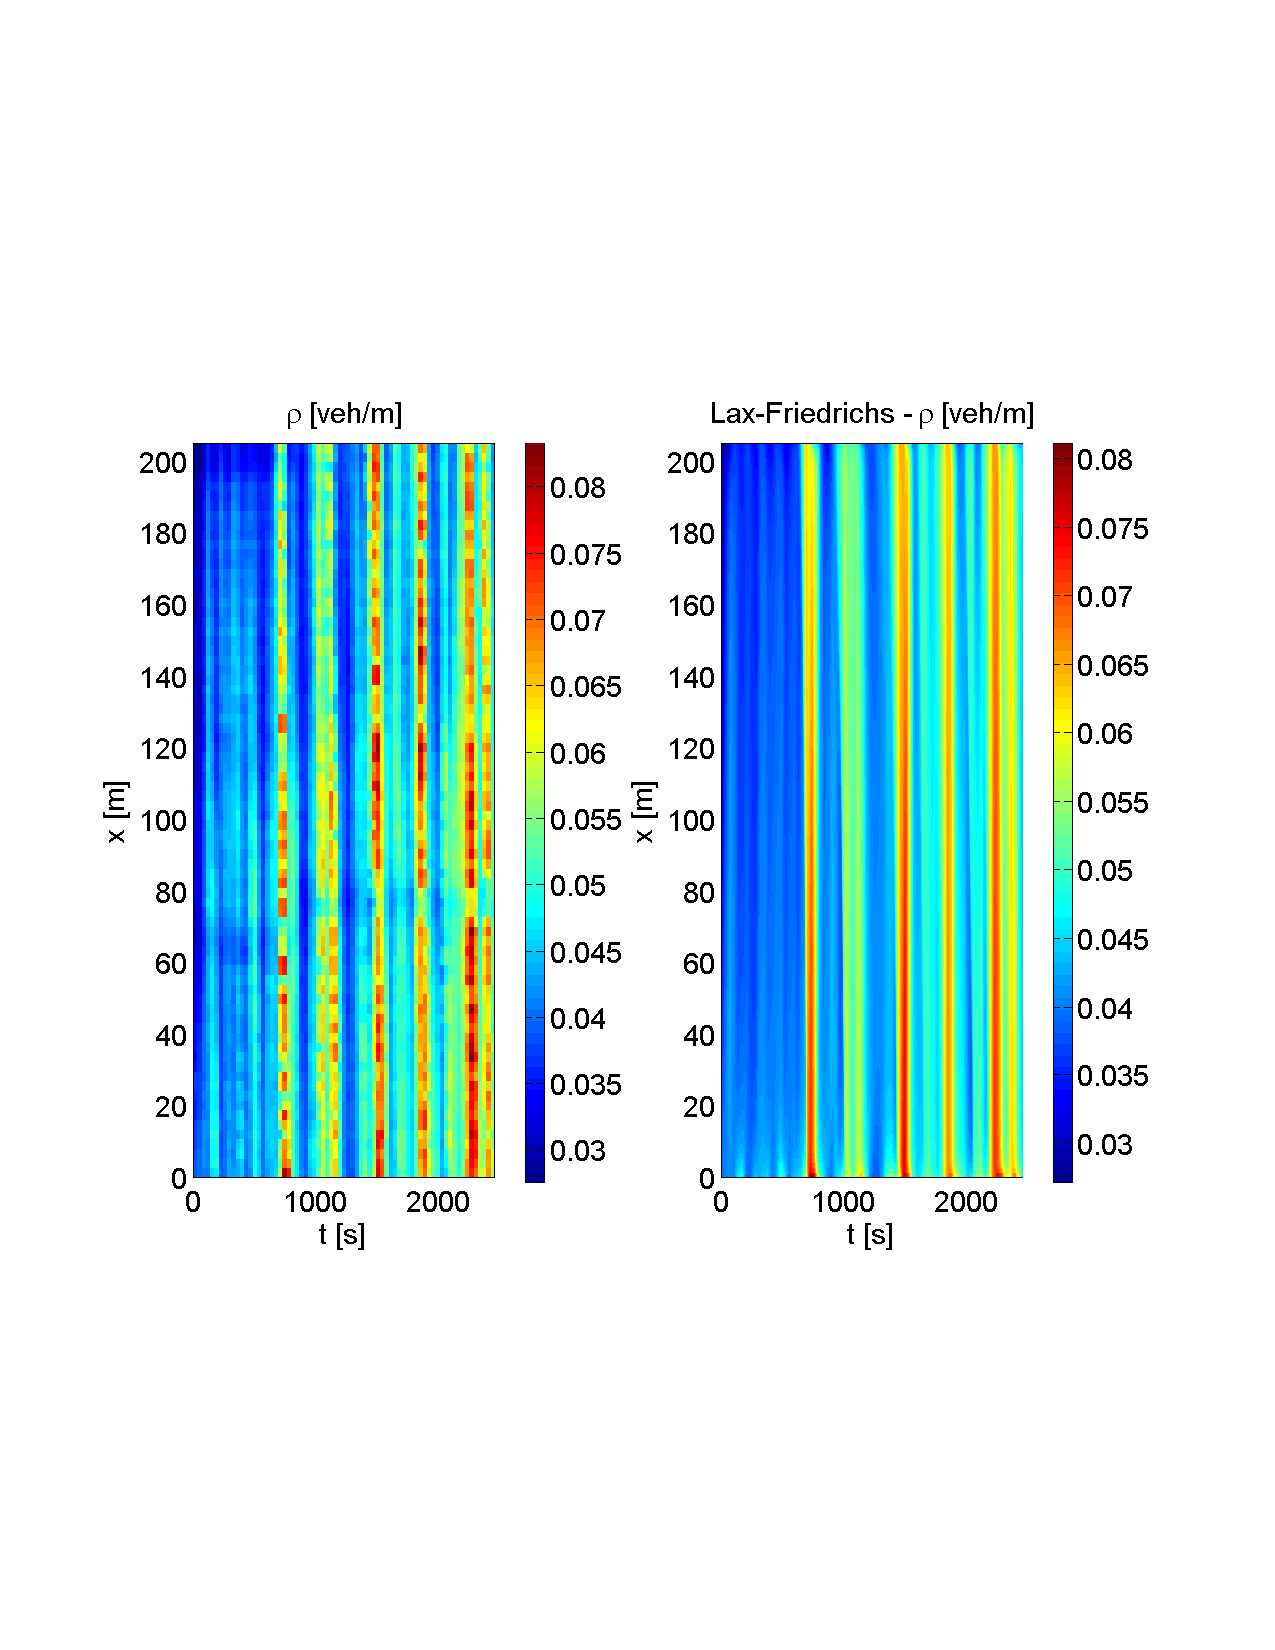
\includegraphics[trim = 20mm 75mm 20mm 75mm, width = 100mm, height = 60mm]{LFrho.pdf}
\caption{Lax-Friedrichs scheme.}
\label{fig:LFrho}
\end{figure}

\begin{figure}[H]
\centering
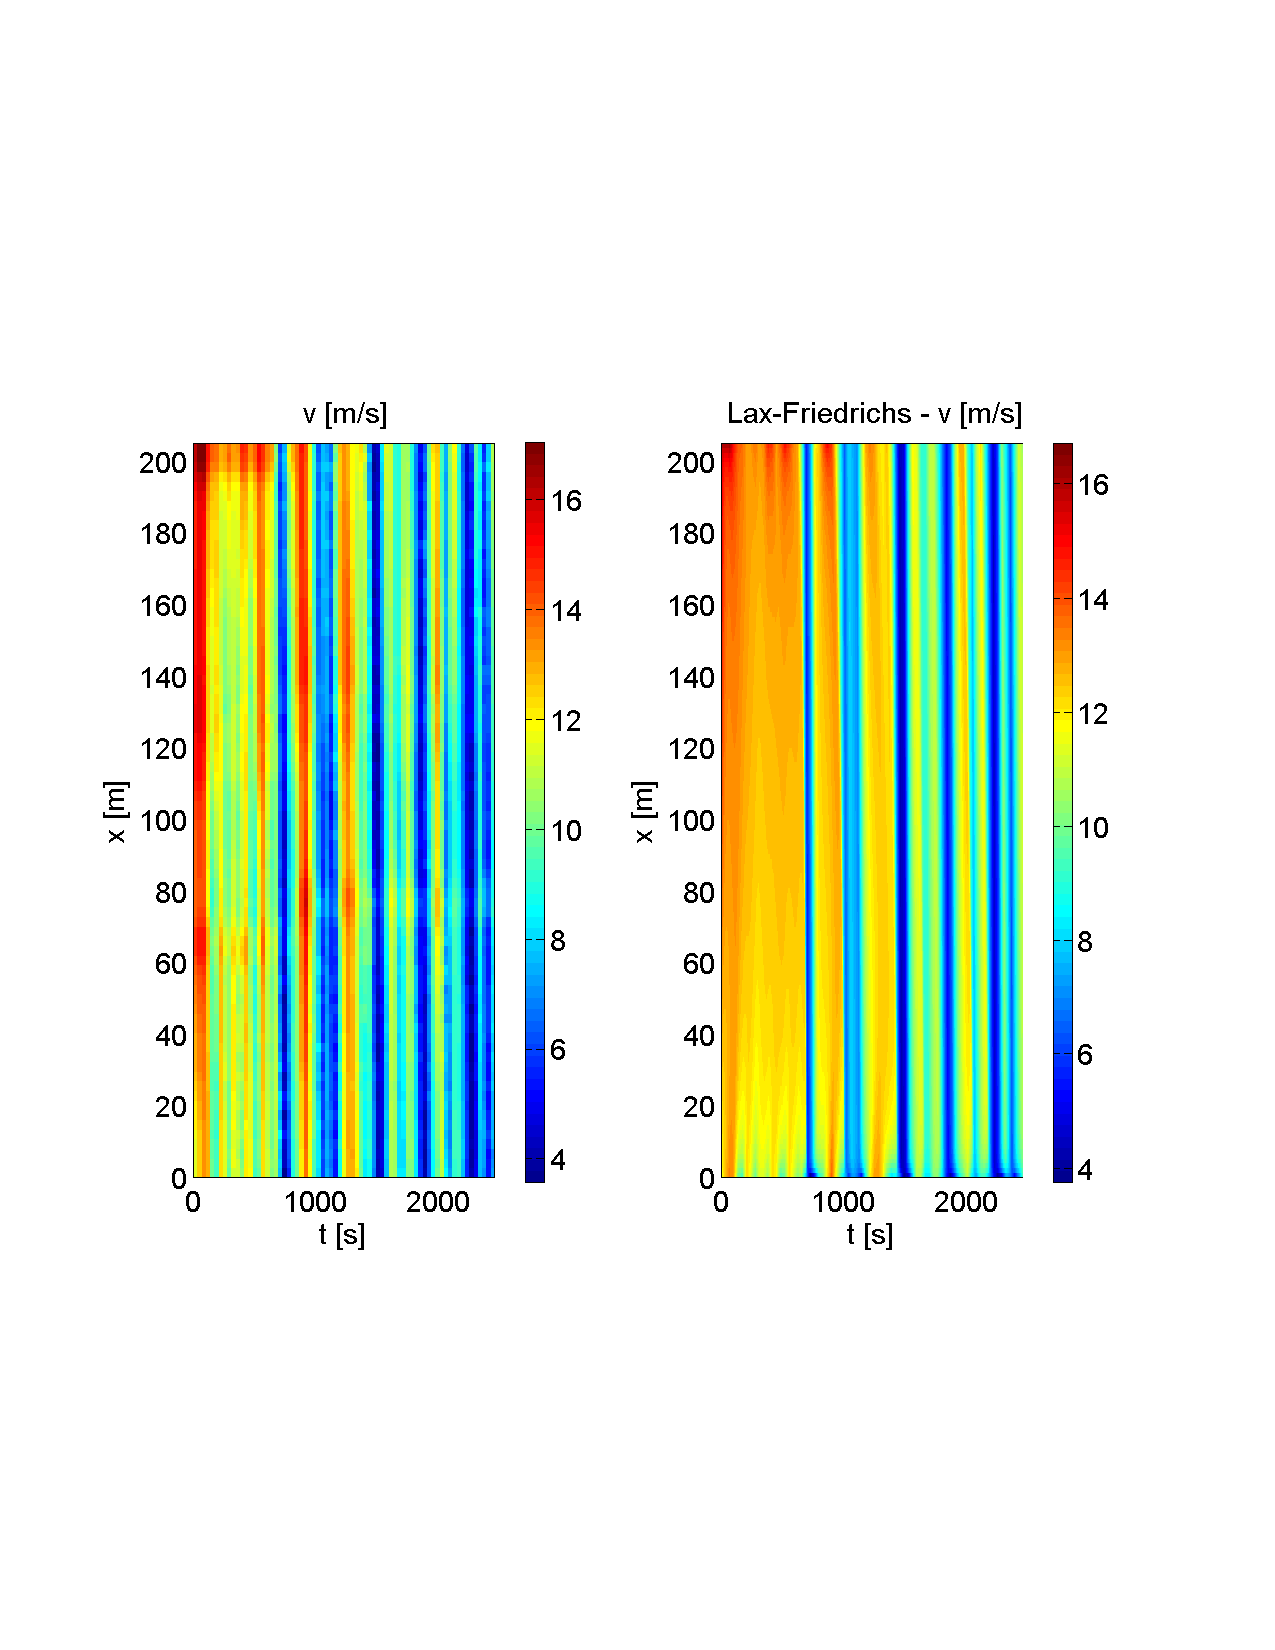
\includegraphics[trim = 20mm 75mm 20mm 75mm, width = 100mm, height = 60mm]{LFv.pdf}
\caption{Lax-Friedrichs scheme.}
\label{fig:LFv}
\end{figure}

\begin{figure}[H]
\centering
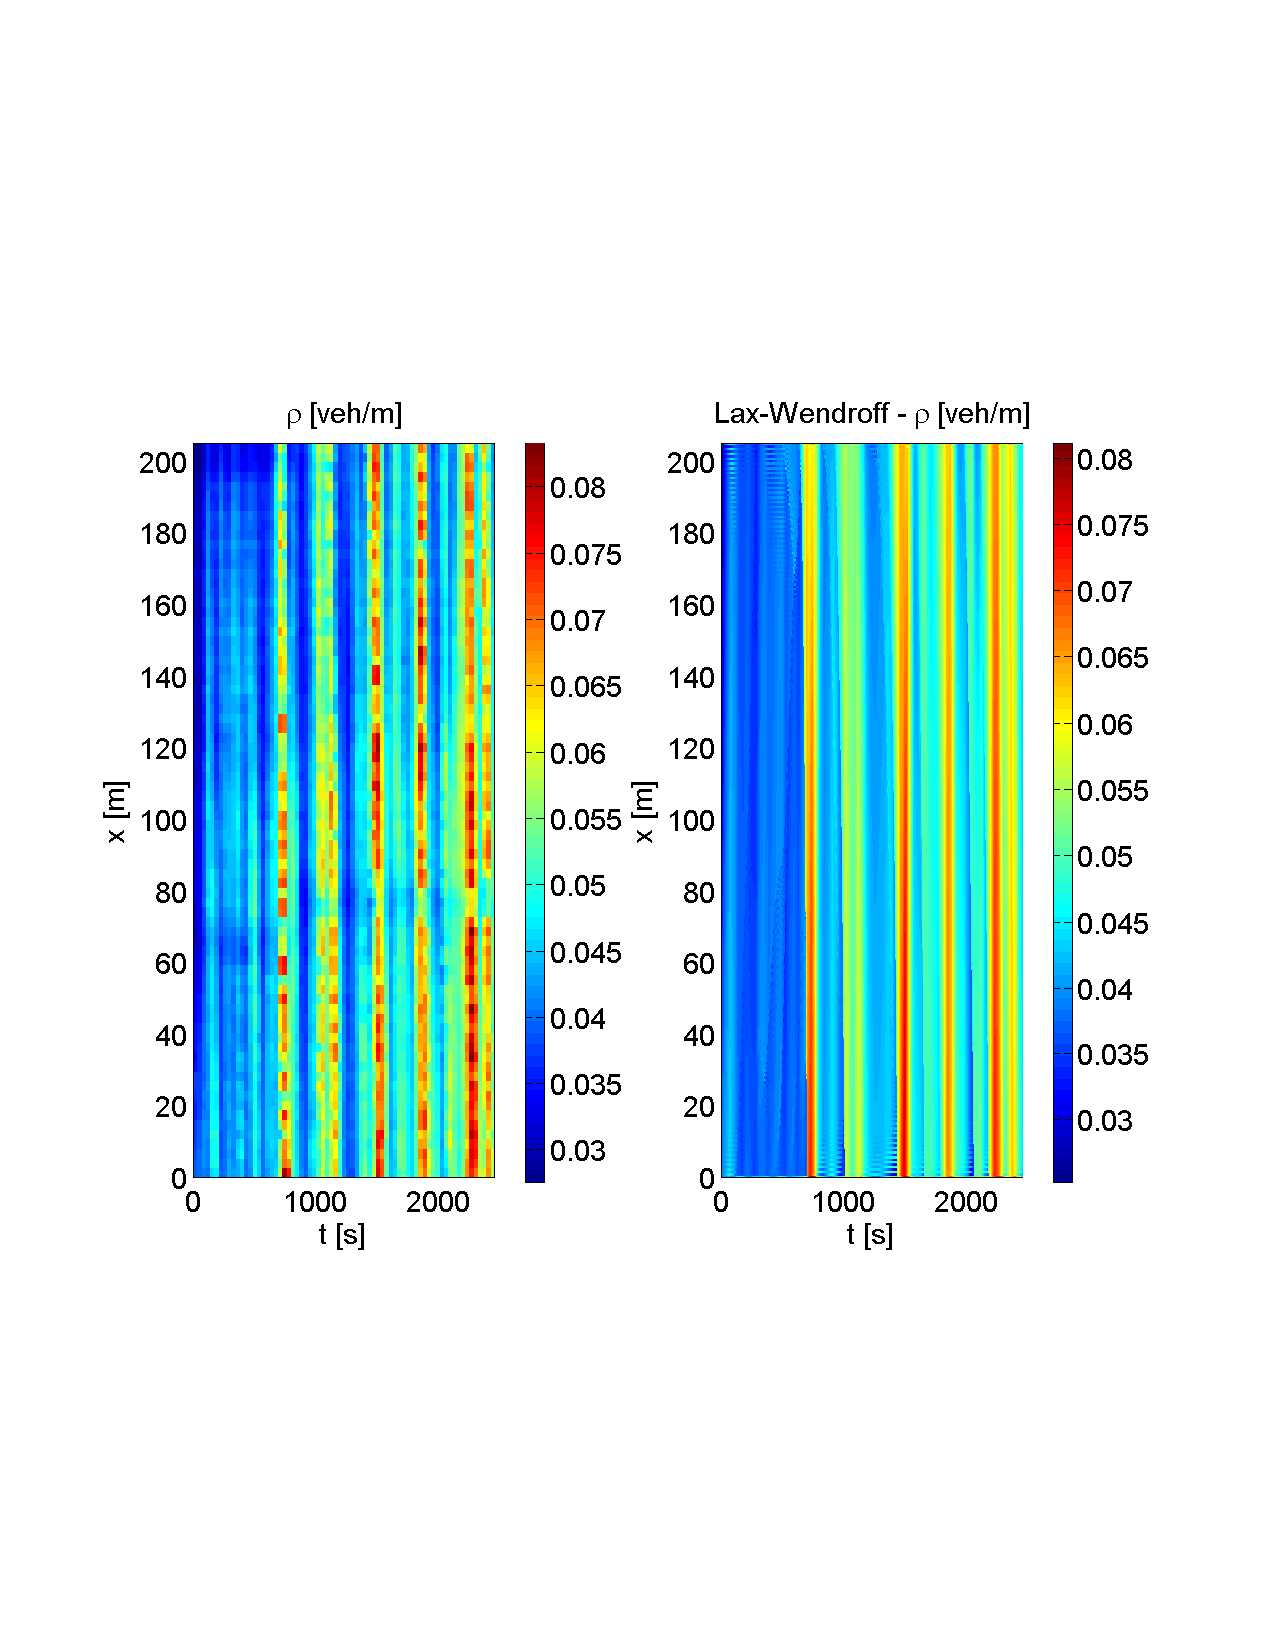
\includegraphics[trim = 20mm 75mm 20mm 75mm, width = 100mm, height = 60mm]{LWrho.pdf}
\caption{Lax-Wendroff scheme.}
\label{fig:LWrho}
\end{figure}

\begin{figure}[H]
\centering
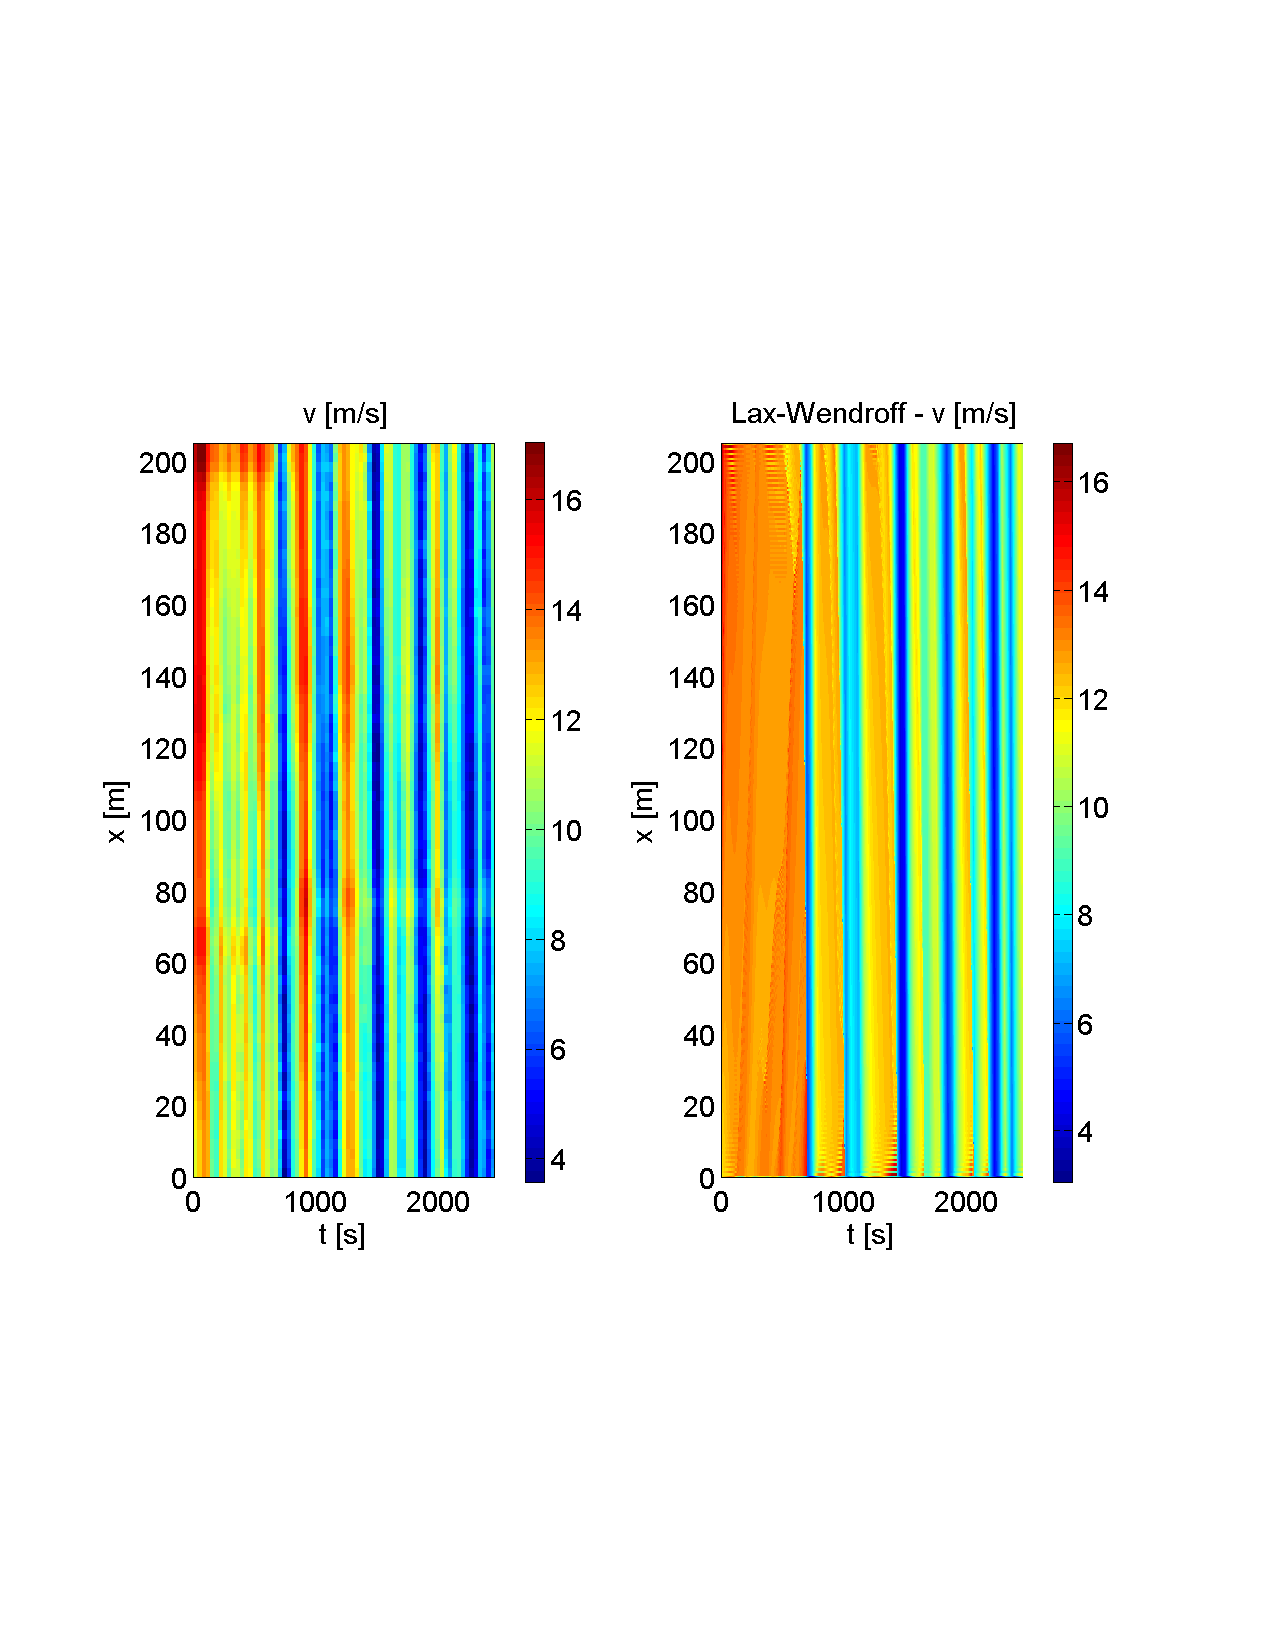
\includegraphics[trim = 20mm 75mm 20mm 75mm, width = 100mm, height = 60mm]{LWv.pdf}
\caption{Lax-Wendroff scheme.}
\label{fig:LWv}
\end{figure}

\section{Implicit schemes}

We apply the following implicit schemes on the linearized ARZ equation. 

\subsection{Crank-Nicolson}

For a PDE system of the form $U_t + A U_x = 0$, the Crank-Nicolson scheme is
\begin{equation}
\dfrac{U_j^{n+1} - U^n_j}{\Delta t} = -\dfrac{A}{2} (D^0_x u^n_j + D^0_x U^{n+1}_j).
\end{equation}
Letting $R = A \dfrac{\Delta t}{\Delta x}$, we can rearrange to write

\begin{equation}
\dfrac{1}{4}R U^{n+1}_{j+1} + U^{n+1}_j - \dfrac{1}{4}R U^{n+1}_{j-1} =  -\dfrac{1}{4}R U^{n}_{j+1} + U^{n}_j + \dfrac{1}{4}R U^{n}_{j-1}.
\end{equation}

We can also write

\begin{equation}
\underbrace{\begin{bmatrix}
1 & \dfrac{1}{4}R & 0 \cdots \\
-\dfrac{1}{4}R & \ddots & \ddots \\
0 & \ddots \\
\vdots & & &
\end{bmatrix}}_{A_1} 
\begin{bmatrix}
U^{n+1}_1 \\ U^{n+1}_2 \\ U^{n+1}_3 \\ \vdots \\ 
\end{bmatrix} = 
\underbrace{\begin{bmatrix}
1 & -\dfrac{1}{4}R & 0 \cdots \\
\dfrac{1}{4}R & \ddots & \ddots \\
0 & \ddots \\
\vdots & & &
\end{bmatrix}}_{A_2}  
\begin{bmatrix}
U^{n}_1 \\ U^{n}_2 \\ U^{n}_3 \\ \vdots \\ 
\end{bmatrix}.
\end{equation}
Then solving the scheme essentially involves inverting a matrix:

\begin{equation}
\textbf{U}^{n+1} = A_1^{-1}A_2 \textbf{U}^n.
\end{equation}

\begin{figure}[H]
\centering
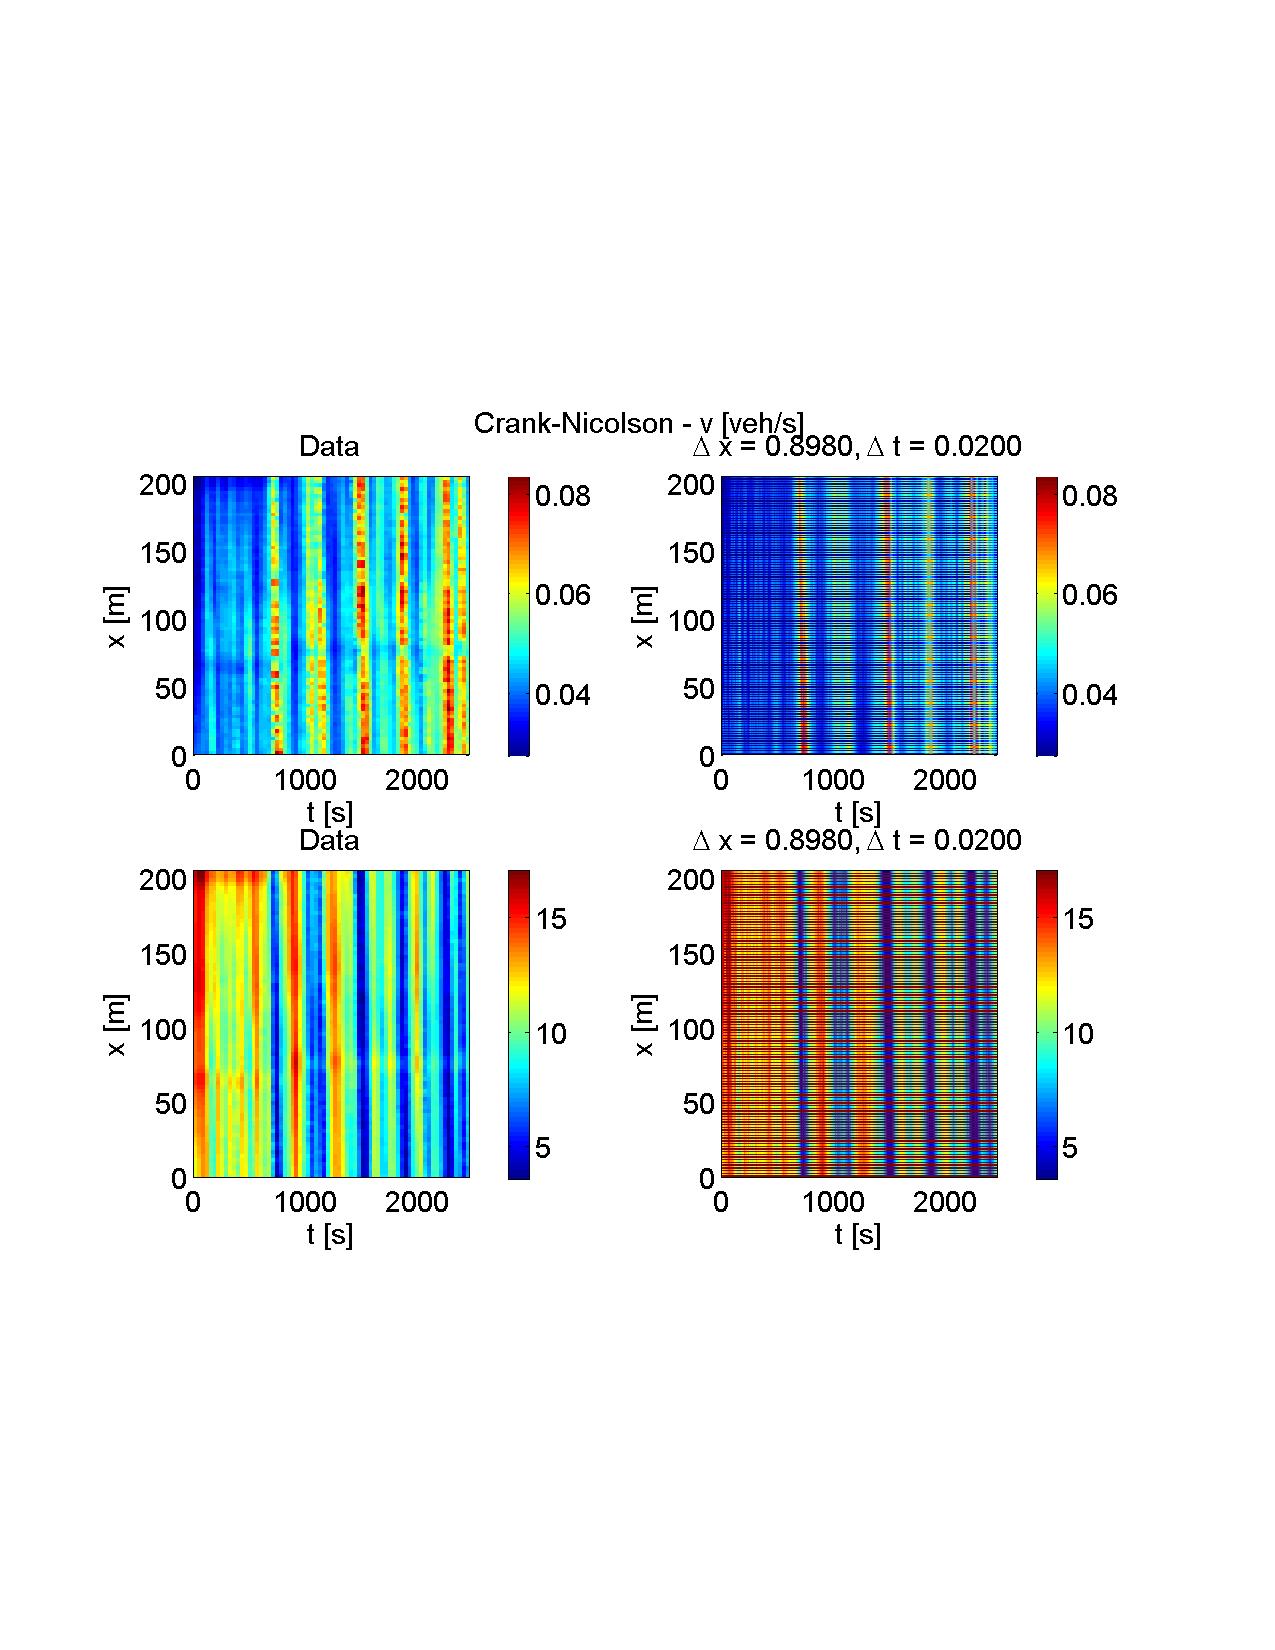
\includegraphics[trim = 50mm 70mm 50mm 65mm, width = 120mm, height = 140mm]{CNrhov_dx_3_dt_45.pdf}
\caption{Although the Crank-Nicolson scheme is stable, it produces spurious oscillations. 
}
\label{fig:CNrho}
\end{figure}


\bibliographystyle{ieeetr}
\bibliography{mybibfile}


\end{document}